% ai-phishing-detection-dissertation/report/sections/4-results/xai-for-random-forest-using-shap/local-explanations-instance-level.tex

\subsubsection*{Local explanations (instance-level)}
SHAP was also used to generate local explanations for a few individual email predictions. It shows a more detailed, yet refined view on how each feature for a specific instance contributed to a certain classification outcome. Waterfall plots were generated for a few selected examples from the test set.\newline

\noindent Instance 0: Correctly classified legitimate email (ham)

\begin{itemize}
  \item \textbf{Original text snippet (instance 0)}: "\textit{attached is the "final" counterparty matrix that is going to be uploaded into eol. please carefully review the tab that corresponds to your area of expertise (i.e. credit, legal, tax, contracts) or th}"
  \item \textbf{Model prediction}:
  \begin{itemize}
    \item \textit{True label}: 0 (Ham)
    \item \textit{Predicted label}: 0 (Ham)
    \item \textit{Predicted probability (phishing)}: 0.0334
  \end{itemize}
\end{itemize}

\begin{figure}[H]
  \begin{center}
    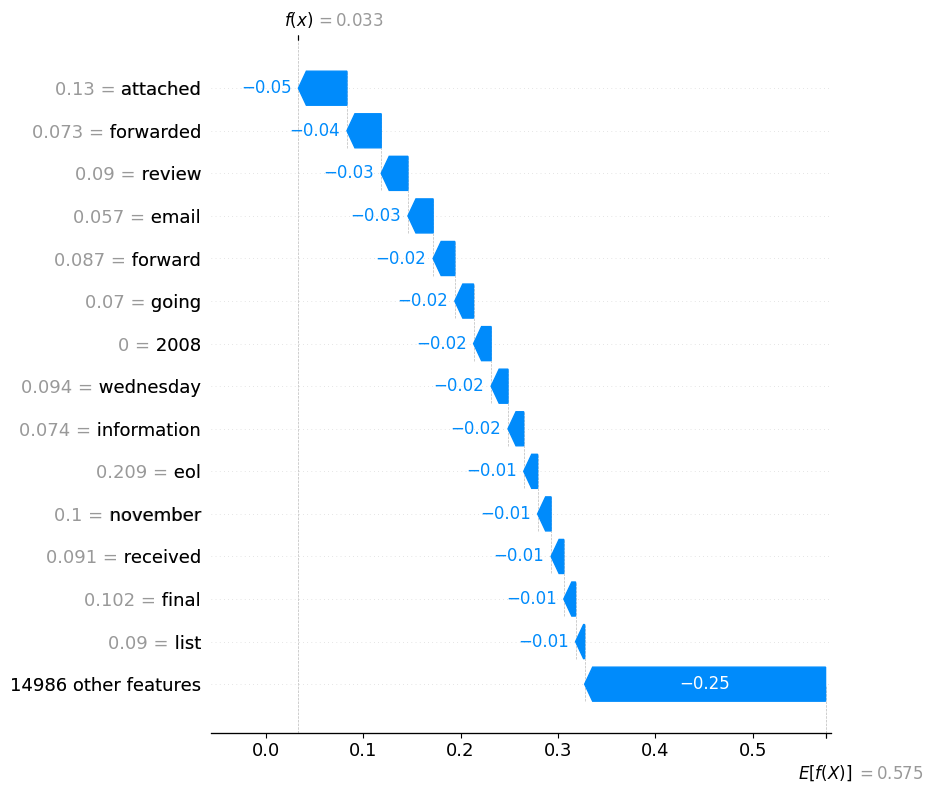
\includegraphics[scale=0.85]{xai-visualisations/random-forest/shap-local-explanations.png}
    \caption{SHAP waterfall plot instance 0}
  \end{center}
\end{figure}

\noindent The above figure shows the SHAP waterfall plot for a correct model classification for a legitimate email (ham) with a low probability of being a phishing email, \textbf{0.0034}. The plot show that the most influential features, "\textit{attached}", "\textit{forwarded}", and "\textit{review}", are consistent with the tone of the email content. On the other hand, features with smaller SHAP values, such as "final" or "list" had little impact on the classification. \newline

\noindent Instance 1: Correctly classified phishing email (moderate confidence)

\begin{itemize}
  \item \textbf{Original text snippet (instance 1)}: "\textit{so many parents has many benefits. report says.at the beach her kids it's chasing butterflies, playing withis an important one," said dr. kenneth many parentsand parents alike. one day a week. contrib}"
  \item \textbf{Model prediction}:
  \begin{itemize}
    \item \textit{True label}: 1 (Phishing)
    \item \textit{Predicted label}: 1 (Phishing)
    \item \textit{Predicted probability (phishing)}: 0.5192
  \end{itemize}
\end{itemize}

\begin{figure}[H]
  \begin{center}
    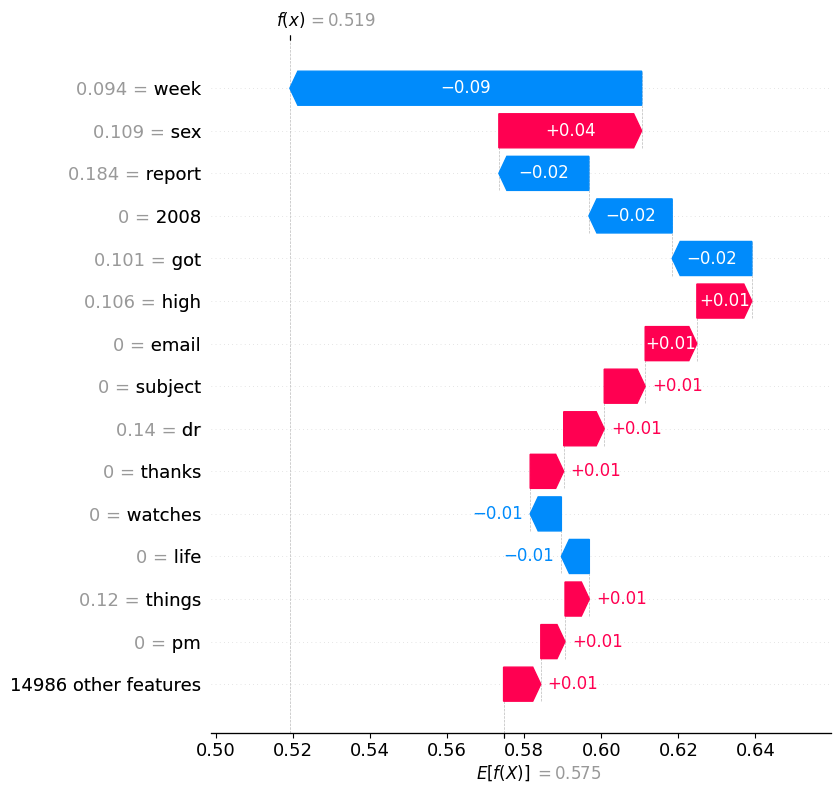
\includegraphics[scale=0.85]{xai-visualisations/random-forest/shap-global-feature-importance-2.png}
    \caption{SHAP waterfall plot instance 1}
  \end{center}
\end{figure}

\noindent The SHAP waterfall plot for this instance shows a correct model classification for an identified phishing email, with a phishing probability of \textbf{0.5192}. The features "\textit{week}", "\textit{sex}", and "\textit{report}", contributed the most to the overall classification. The net positive of all the Shapley value scores add to a positive score, i.e. the email instance is phishing.\newline

\noindent Instance 2: Correctly classified phishing email (high confidence)

\begin{itemize}
  \item \textbf{Original text snippet (instance 2)}: "\textit{b zqq u nn y dr hh u vuw gs on psk line fa lwh st ship zg ping. us licens bmh ed. overnight ship hgm ping. gr of eat pric aw es.}"
  \item \textbf{Model prediction}:
  \begin{itemize}
    \item \textit{True label}: 1 (Phishing)
    \item \textit{Predicted label}: 1 (Phishing)
    \item \textit{Predicted probability (phishing)}: 0.9750
  \end{itemize}
\end{itemize}

\begin{figure}[H]
  \begin{center}
    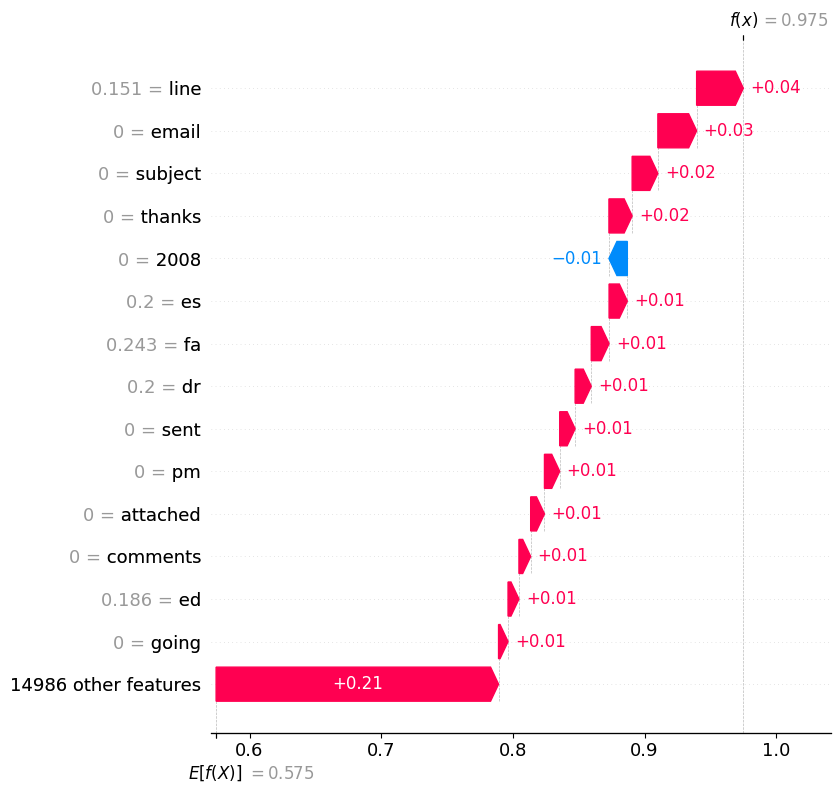
\includegraphics[scale=0.85]{xai-visualisations/random-forest/shap-global-feature-importance-3.png}
    \caption{SHAP waterfall plot instance 2}
  \end{center}
\end{figure}

\noindent This email instance was classified with high confidence as a phishing email, with nearly all of the features having a positive Shapley value, contributing to a correctly classified phishing email with a predicted probability of \textbf{0.9760}. The features "\textit{line}", "\textit{email}", and "\textit{subject}" were the most influential in this classification, indicating that the model identified key terms associated with phishing emails.\newline
